\documentclass[final,hyperref={pdfpagelabels=false}]{beamer}
\usepackage{grffile}
\mode<presentation>{\usetheme{PosterLogProb}}
%\mode<presentation>{\usetheme{I6pd2}}
\usepackage[english]{babel}
\usepackage[latin1]{inputenc}
\usepackage{amsmath,amsthm, amssymb, latexsym}
\usepackage{epsfig}
\usepackage{listings}
\usepackage{lstlinebgrd}

%\usepackage{algorithm}
%\usepackage{algorithmic}

%\usepackage{times}\usefonttheme{professionalfonts}  % obsolete
%\usefonttheme[onlymath]{serif}
%\boldmath
\usepackage[orientation=portrait,size=a0,scale=1.4,debug]{beamerposter}
% change list indention level
% \setdefaultleftmargin{3em}{}{}{}{}{}
\providecommand\thispdfpagelabel[1]{}
\setbeamertemplate{bibliography entry title}{\color{black}}
\setbeamertemplate{bibliography entry location}{}
\setbeamertemplate{bibliography entry note}{}


%\usepackage{snapshot} % will write a .dep file with all dependencies, allows for easy bundling

\usepackage{array,booktabs,tabularx}
\newcolumntype{Z}{>{\centering\arraybackslash}X} % centered tabularx columns
\newcommand{\pphantom}{\textcolor{ta3aluminium}} % phantom introduces a vertical space in p formatted table columns??!!

\listfiles

\usepackage{amsthm}
%%%%%%%%%%%%%%%%%%%%%%%%%%%%%%%%%%%%%%%%%%%%%%%%%%%%%%%%%%%%%%%%%%%%%%%%%%%%%%%%%%%%%%


 \title{\huge\bfseries\hspace*{-1em} Empurrando Juntos: \\A platform for social participation}
\date{}
\author{\large Tallys Martins
\and Dylan Guedes
\and Luan Guimar�es \\
\and Ricardo Poppi
\and Henrique Parra
\and Paulo Meirelles
}
\institute[UNB/CD]{University of Bras�lia and Cidade Democr�tica NGO, Brazil}

%%%%%%%%%%%%%%%%%%%%%%%%%%%%%%%%%%%%%%%%%%%%%%%%%%%%%%%%%%%%%%%%%%%%%%%%%%%%%%%%%%%%%%
\newlength{\columnheight}
\setlength{\columnheight}{105cm}


%%%%%%%%%%%%%%%%%%%%%%%%%%%%%%%%%%%%%%%%%%%%%%%%%%%%%%%%%%%%%%%%%%%%%%%%%%%%%%%%%%%%%%
\begin{document}
\setbeamertemplate{caption}{\raggedright\insertcaption\par}
\begin{frame}
  \begin{columns}
    % ---------------------------------------------------------%
    % Set up a column 
    \begin{column}{.49\textwidth}
      \begin{beamercolorbox}[center,wd=\textwidth]{postercolumn}
        \begin{minipage}[T]{.95\textwidth}  % tweaks the width, makes a new \textwidth
          \parbox[t][\columnheight]{\textwidth}{ % must be some better way to set the the height, width and textwidth simultaneously
            % Since all columns are the same length, it is all nice and tidy.  You have to get the height empirically
            % ---------------------------------------------------------%
            % fill each column with content
%\vfill

\begin{block}{What is Empujando Juntos}

  \begin{itemize}
    \item Allow people to create online conversations to debate about any subject
    with a different paradigm that we call ``crowdsource``, which fosters
    more engagement than standard models like forum/thread

    \item People can to give their opinion by simple clicking in ``agree``,
    ``disagree`` or ``skip`` in other's comments

    \item Identify different groups of opinion based on the reactions of the
    participants in the comments using clustering algorithms.

    \item Uses Polis engine to calculate the groups. Every opinion is considered,
    majority and minority.

    \item Applying gamification concepts we invented the ``Push`` power. People in
    ownership of this ability are able to send direct messages and create events
    in the platform

    \item The ``Push`` is given to special actors in the groups formed by Polis.
    Three profiles are considered, the activist, the bridge and the consultation
    owner.

    \begin{figure}
      \begin{center}
        \includegraphics[scale=1.3]{../images/userprofiles.png}
        \caption{Profiles identified by Empurrando Juntos}
        \label{fig:background:free-software-repository}
      \end{center}
    \end{figure}
    
  \end{itemize}
\end{block}

\begin{block}{Why Empurrando Juntos?}
  \begin{itemize}
    \item We use the successful concept of conversation brought by Polis and extend it,
    allowing users to have an even more interaction with each other.

    \item  The ``Push`` power aims to foster the discussion between different
    groups of opinion, and increase the engagement of people in terms of social
    participation.
  \end{itemize}
\end{block}

\begin{block}{Empujando Juntos Features}
  \begin{itemize}
    \item Create conversations about any subject
    \item 
  \end{itemize}
\end{block}

\vfill

\begin{block}{System Architecture}
	\begin{itemize}
    \item front-end application, written in React Native\footnote{\url{facebook.github.io/react-native}}
    NodeJS\footnote{\url{nodejs.org/en}} server. The server module is responsible
    for managing users, ``the Push'' resources for the gamification, and to make the
    interface with the external cluster processing service, for which we reverse
    engineered Polis.
  \end{itemize}

  \begin{figure}
    \begin{center}
      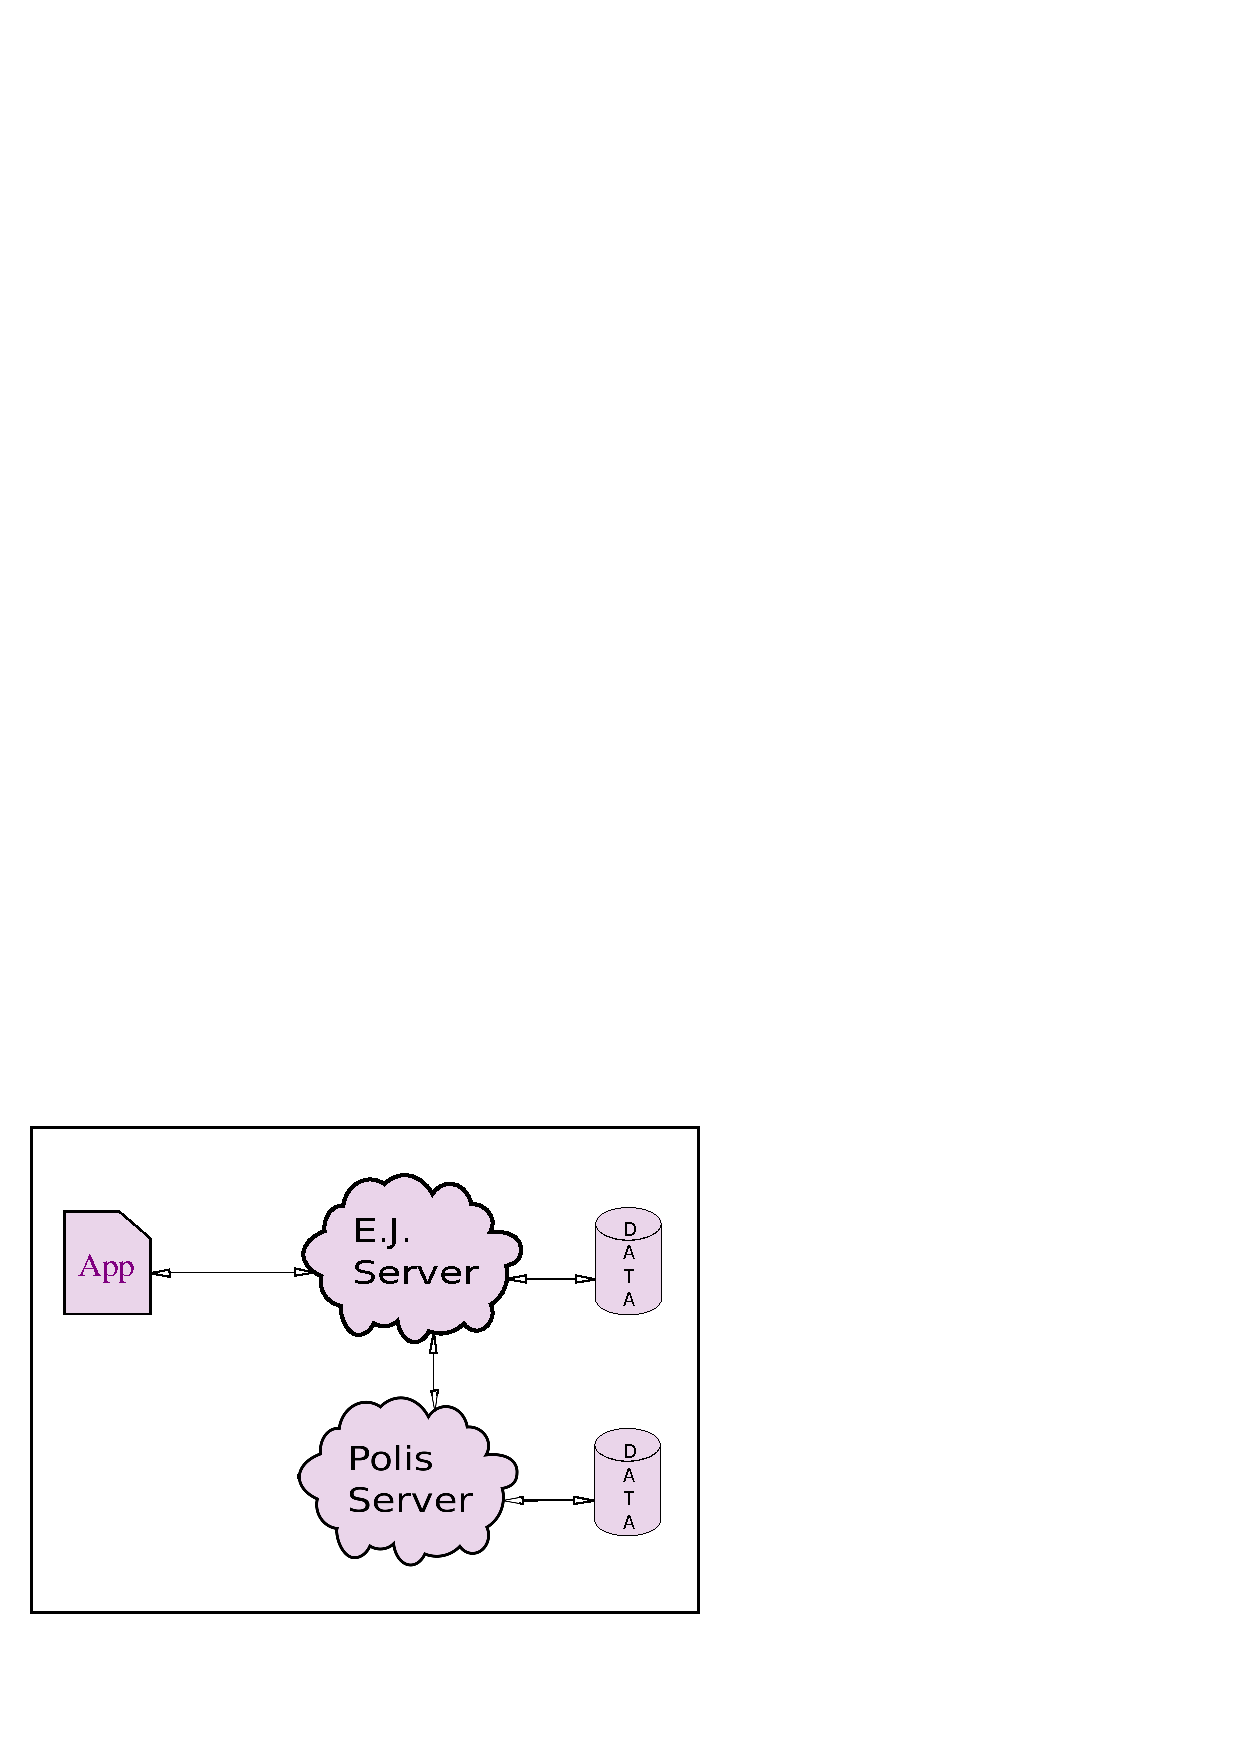
\includegraphics[scale=1.5]{../images/architecture-1.png}
      \caption{Simplified architecture of the system}
      \label{fig:architecture}
    \end{center}
  \end{figure}
\end{block}
\vfill

\begin{block}{Continuous static analysis: kiskadee}

\textit{kiskadee} performs continuous static analysis on software
  repositories. It is extensible regarding what software
  repositories it monitors. For this work we decided to point it to
  GNU/Linux distribution repositories.

  \textit{kiskadee}'s features are described below:

\begin{enumerate}
\item \textbf{Monitor specific software repositories for new releases.} This\
way, we can track and analyze each release of the monitored packages since we\
started monitoring them.

\item \textbf{Download new software packages from the repositories.}

\item \textbf{Run multiple static analyzers on the downloaded packages.}

\item \textbf{Translate each static analyzer report to a common report format.} This\
is needed to enable analyzing the reports during the ranking and visualization\
phase. Since the system is extensible, we do not want to write parsing\
rules for each static analyzer report format to compare the analyzers, so we do\
this before saving the static analysis output.

\item \textbf{Save the reports in a database.}
\end{enumerate}

\end{block}

%-------------------------------------------------------------------------------
\vfill


}
\end{minipage}
\end{beamercolorbox}
\end{column}
% ---------------------------------------------------------%
% end the column

% ---------------------------------------------------------%
% Set up a column 
\begin{column}{.49\textwidth}
  \begin{beamercolorbox}[center,wd=\textwidth]{postercolumn}
    \begin{minipage}[T]{.95\textwidth} % tweaks the width, makes a new \textwidth
      \parbox[t][\columnheight]{\textwidth}{ % must be some better way to set the the height, width and textwidth simultaneously
        % Since all columns are the same length, it is all nice and tidy.  You have to get the height empirically
        % ---------------------------------------------------------%
        % fill each column with content

\begin{block}{Continuous static analysis: kiskadee}
\begin{figure}[!h]
  \centering
  \includegraphics[width=.95\textwidth]{figures/ej_overview} 
  \caption{kiskadee strategy overview.}
  \label{fig:kiskadee_overview} 
\end{figure}

Finally, the static analysis reports in the database are ranked with using a model based on a boosting algorithm.

\end{block}

\vfill

\begin{block}{Training our learning model with Juliet}

  To train our model, we use Juliet , a static analysis test suit with injected software flaws (\textbf{CWEs}).

  \begin{itemize}
    \item Test suite with $61,387$ test cases.
    \item $118$ different CWEs.
    \item Each test case is a file with C programming language code
    \begin{itemize}
      \item with a specific flaw (\textbf{location known})
      \item and a similar code snippet without the flaw.
    \end{itemize}
  \end{itemize}
\end{block}

\vfill

%\begin{block}{\textit{A static analysis report sample}}
  %\lstinputlisting[language={},basicstyle=\ttfamily\tiny]{reports/sample.txt}
%\end{block}

%\vfill

\begin{block}{Ranked static analysis report}
  \lstset{
    linebackgroundcolor={\color{green!\the\numexpr 17-\value{lstnumber}\relax}},
  }
  \lstinputlisting[language={},basicstyle=\ttfamily\tiny]{reports/ranked.txt}
\end{block}

\vfill

\begin{block}{Reports for different versions}

  Since we analyze different versions of the same software, it would be
  interesting to provide a list containing only the warnings introduced in a
  specific software version.

  \begin{columns}[T] % contents are top vertically aligned
     \begin{column}[T]{0.45\textwidth} % each column can also be its own environment
    \lstset{
         linebackgroundcolor={\color{yellow}},
       }
      \lstinputlisting[title=foo-v1.0,language={},basicstyle=\ttfamily\tiny]{reports/v1.txt}
     \end{column}
     \begin{column}[T]{0.55\textwidth} % alternative top-align that's better for graphics
  \lstset{
       linebackgroundcolor={\ifodd\value{lstnumber}\color{yellow}\else\color{green}\fi},
     }
      \lstinputlisting[title=foo-v1.1, language={},basicstyle=\ttfamily\tiny]{reports/v2.txt}
     \end{column}
     \end{columns}

     We compare the warnings generated in a software previous version with the
     ones for the current version and display only the warnings introduced in
     the current version. Related works mention that warnings that persist
     through different software versions tend to be false positives.

%\end{block}
%\begin{block}{Reports delta for different versions}
    \lstset{
         linebackgroundcolor={\color{green}},
       }
  \lstinputlisting[title=v1.1 - v1.0,language={},basicstyle=\ttfamily\tiny]{reports/diff.txt}
\end{block}
             
  \vfill

  \begin{block}{Current Status and Future Work}
    \begin{itemize}
      \item This is an ongoing research. Currently, we are preparing the first kiskadee
    release (v0.1), to perform analysis on C/C++ packages of the Debian
    GNU/Linux distribution using cppcheck, flawfinder and Frama-C.

  \item In the future, we want to extend kiskadee to monitor other software
    repositories, such as SourceForge and git repositories. We also want to
    improve the approach to handle persistent warnings (generated in previous
    versions) by assigning them a lower grade during the classification process
    instead of just omitting them.

  \item kiskadee development is open and can be found in \url{gitlab.com/kiskadee}.
    \end{itemize}
  \end{block}


      }
      % ---------------------------------------------------------%
      % end the column
        \end{minipage}
      \end{beamercolorbox}
    \end{column}
    % ---------------------------------------------------------%
    % end the column
  \end{columns}
  %\vskip1ex
  % \tiny\hfill\textcolor{ta2gray}{Created with \LaTeX \texttt{beamerposter}  \url{http://www-i6.informatik.rwth-aachen.de/~dreuw/latexbeamerposter.php}}
  
\end{frame}
\end{document}


%%%%%%%%%%%%%%%%%%%%%%%%%%%%%%%%%%%%%%%%%%%%%%%%%%%%%%%%%%%%%%%%%%%%%%%%%%%%%%%%%%%%%%%%%%%%%%%%%%%%
%%% Local Variables: 
%%% mode: latex
%%% TeX-PDF-mode: t
%%% End:

% LocalWords:  ABox ABoxes PSAT
